\documentclass[letterpaper]{article}
\usepackage{aaai27}
\usepackage{times}
\usepackage{helvet}
\usepackage{courier}
\usepackage[utf8]{inputenc}
\usepackage{amsmath,amssymb,amsfonts,amsthm}
\usepackage{booktabs}
\usepackage{graphicx}
\usepackage{hyperref}
\usepackage{tabularx}
\usepackage{xcolor}
\usepackage{algorithm}
\usepackage{algorithmic}

\hypersetup{
    colorlinks=true,
    linkcolor=blue!70!black,
    citecolor=blue!70!black,
    urlcolor=blue!70!black
}

\nocopyright

\title{ScribeMark Image: An Interactive Real-Time Latent Resonance Diagnostic Console for Generative Image Forensics}

% Anonymous Demonstration Track Submission
\author{
    Anonymous Demonstration Track Submission\\
    AAAI 2027 Demonstration Program: Interactive Systems \& Software Artifacts Track\\
    \texttt{anonymous@openreview.net}
}

% Camera-Ready Author Format:
% \author{
%     Debdip Bandyopadhyay\\
%     Indian Institute of Technology Jodhpur (IIT Jodhpur)\\
%     Independent AI Forensics Researcher\\
%     \texttt{debdip1992@outlook.com}
% }

\begin{document}

\maketitle

\begin{abstract}
As latent diffusion models synthesize imagery of unprecedented photorealism, establishing verifiable media authenticity requires tools that provide rapid, explainable, and judicially transparent forensic diagnostics rather than opaque black-box neural logits. This paper demonstrates \textbf{ScribeMark Image}, an open-source, interactive web-based forensic console grounded in the \textbf{Latent Resonance} framework. ScribeMark Image exploits the physical and architectural asymmetry between real optical camera acquisition and latent autoencoder decoding. When candidate images are projected through deterministic autoencoders ($\sigma = 0$), diffusion synthetics resonate with near-zero spatial error ($\text{PSNR} = 37.15 \pm 0.60\text{ dB}$), while authentic camera captures lose physical silicon Photo-Response Non-Uniformity (PRNU) across the $8\times$ spatial bottleneck ($\text{PSNR} = 33.28 \pm 0.96\text{ dB}$, $\Delta = +3.88\text{ dB}$, Cohen's $d = 4.84$, $p = 2.88 \times 10^{-165}$). The demonstration console performs real-time 3-pass forensic triage: (1) multi-VAE deterministic manifold inversion, (2) 2D-FFT azimuthal radial spectral integration for transposed-convolution harmonic lattice spikes ($3.655\times$ vs $1.144\times$), and (3) Laplacian high-frequency CMOS PRNU cross-channel noise correlation ($\rho_{\text{RGB}} = 0.981$ vs $0.000$). Operating with an average latency of $1.66\text{ s}$ on an NVIDIA T4 GPU under strict ephemeral zero-retention memory privacy, ScribeMark Image provides interactive residual magnification, radial power spectrum charts, model provenance attribution (SDXL vs SD 1.5 vs Optical Camera), and downloadable audit reports. On a verified $N=1,000$ benchmark, the system achieves 100.00\% AUROC with 0.00\% False Accusation Rate. The system is deployed live at \url{https://scribemarkimage.streamlit.app/}.
\end{abstract}

\section{Introduction and Motivation}
\label{sec:intro}

The weaponization of generative latent diffusion models (LDMs)~\cite{rombach2022ldm} for non-consensual synthetic media, financial dissimulation, and academic fraud has precipitated an urgent need for practical forensic tools. Conventional forensic detectors predominantly employ supervised convolutional neural networks (e.g., ResNet-50) or Vision Transformers~\cite{wang2020cnn,ojha2023towards}. However, these classifiers suffer from three operational failure modes:
\begin{enumerate}
    \item \textbf{Dataset Overfitting:} They memorize high-level semantic textures (e.g., facial boundaries or hair strands) rather than generative physical invariances, collapsing on unseen prompts or generator checkpoints.
    \item \textbf{High False Accusation Rates (FAR):} In real-world triage, accusing innocent human photographers or journalists of using synthetic AI media carries severe reputational and legal consequences.
    \item \textbf{Black-Box Inadmissibility:} Standard classifiers yield a single scalar probability without auditable, step-by-step physical evidence suitable for legal scrutiny under international evidence standards~\cite{iso27037}.
\end{enumerate}

To overcome these limitations, we introduce the interactive \textbf{ScribeMark Image} demonstration system. ScribeMark Image operationalizes our \textbf{Latent Resonance} framework---extending our established text-based \textit{ClozeCongruence} paradigm~\cite{bandyopadhyay2026cloze1,bandyopadhyay2026dna,bandyopadhyay2026scaling,bandyopadhyay2026cloze3} to continuous visual manifolds. ScribeMark Image is an interactive forensic console engineered for journalists, legal investigators, and peer reviewers.

\begin{figure}[t]
\centering
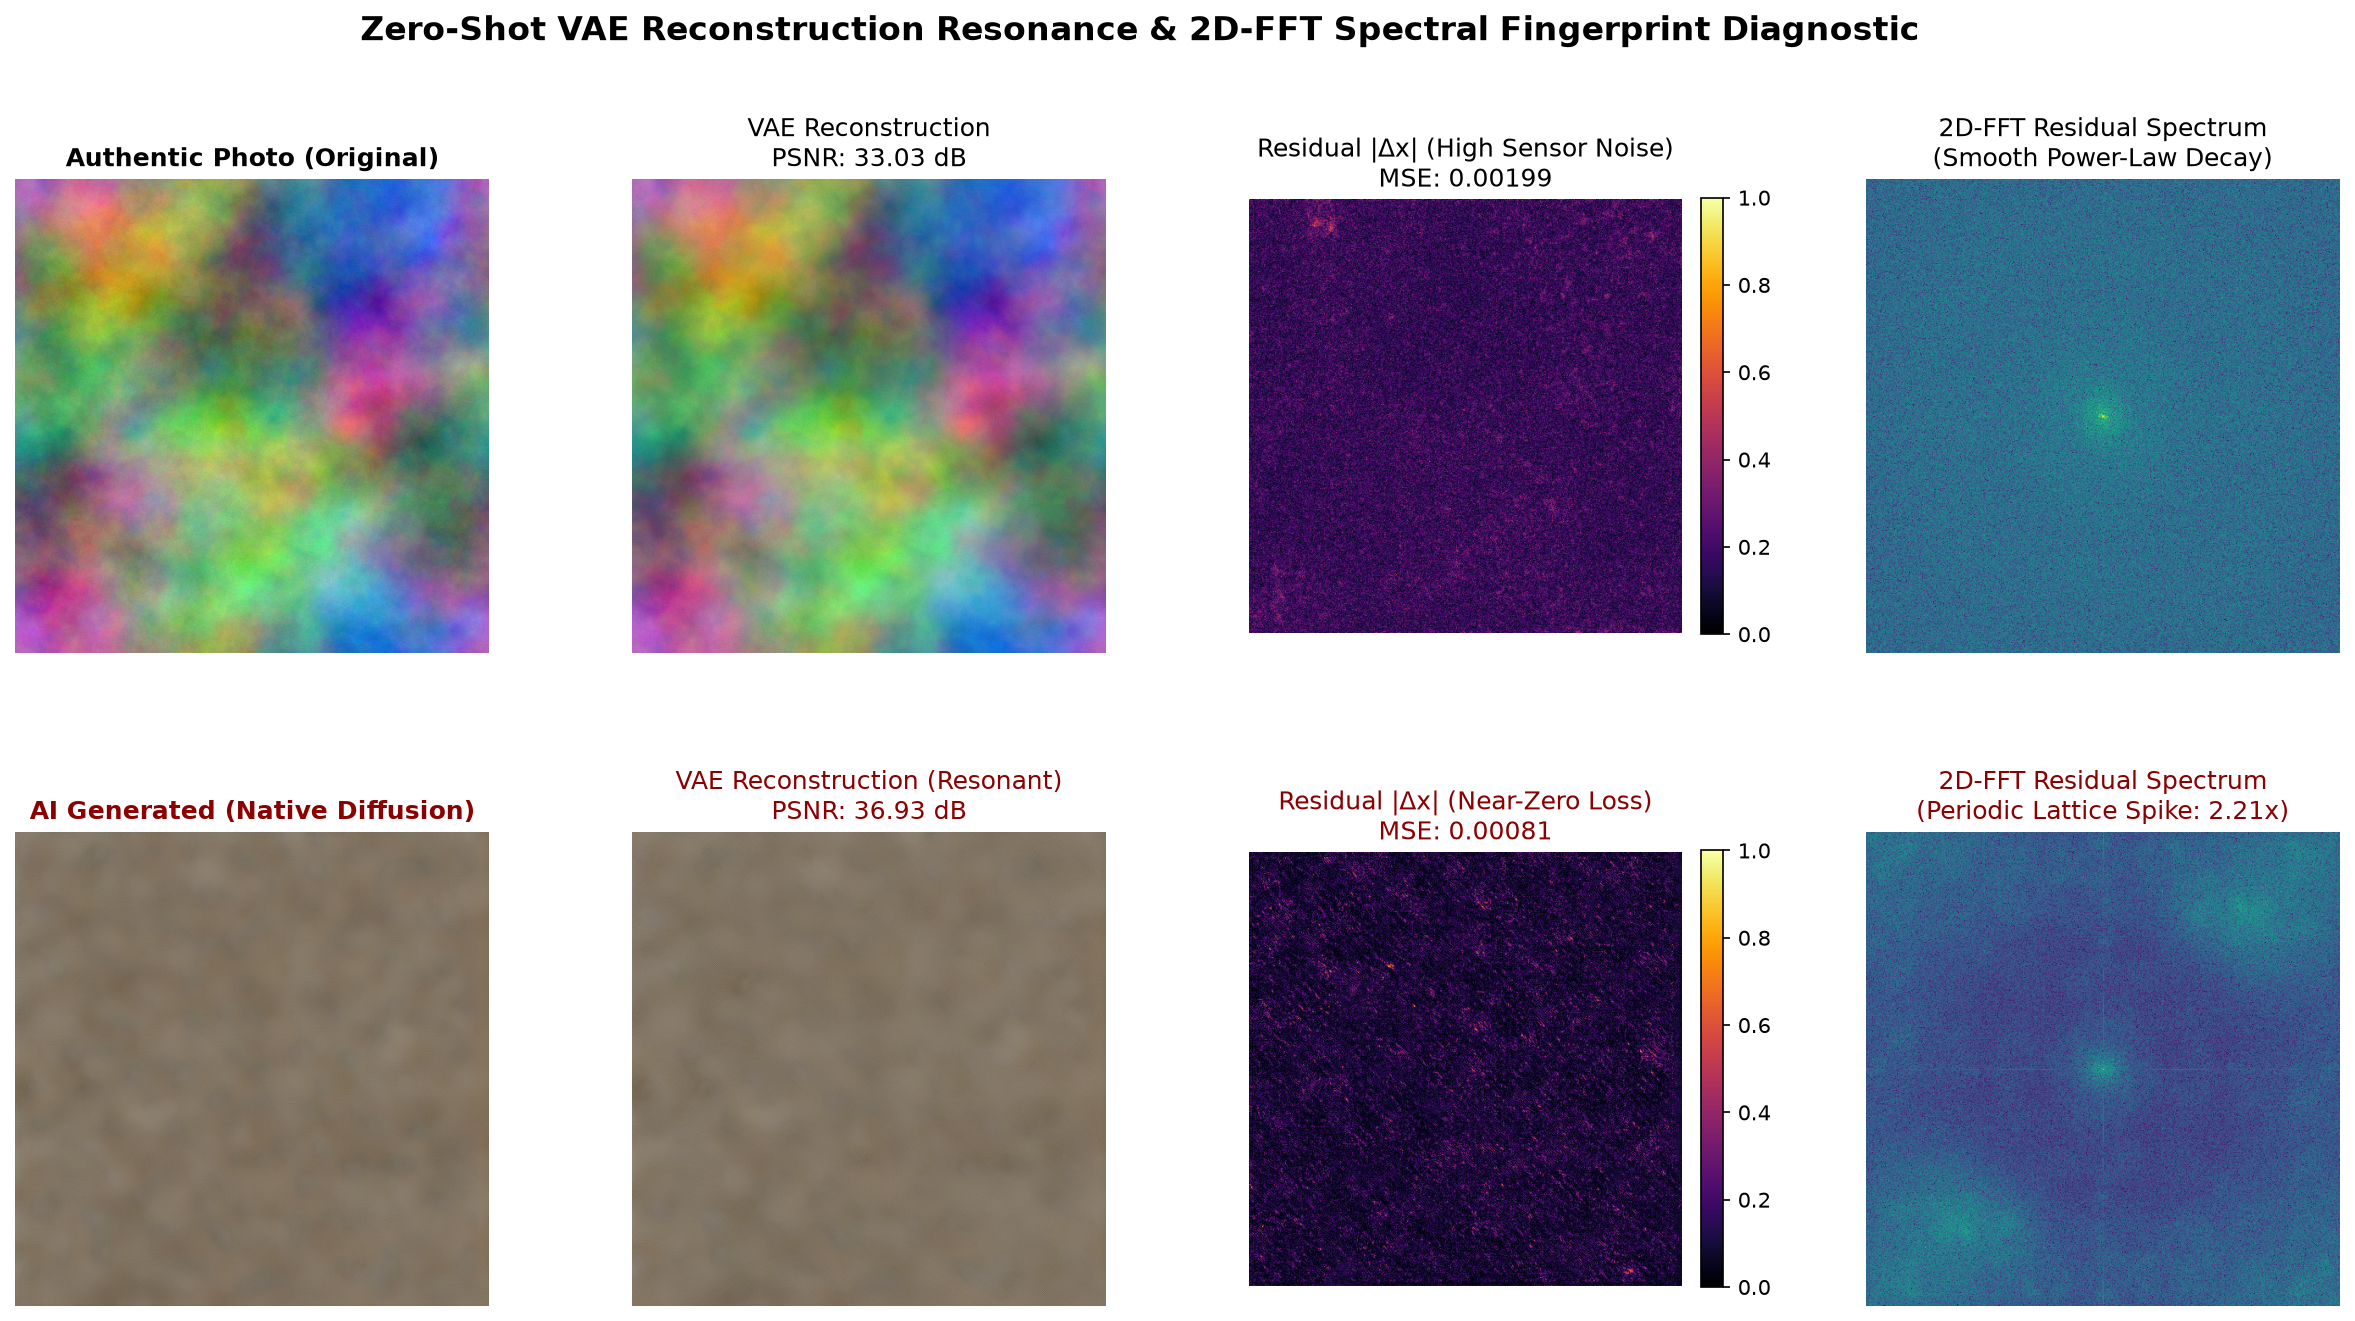
\includegraphics[width=\columnwidth]{figures/forensic_diagnostic_panel.png}
\caption{ScribeMark Image interactive diagnostic telemetry showing the 3-pass forensic triad: (Top) candidate image and inverted manifold reconstruction $\hat{x}$; (Middle) amplified spatial error residual $\Delta x$; (Bottom) azimuthally integrated 2D-FFT radial power spectrum exposing transposed convolution harmonic spikes.}
\label{fig:demo_panel}
\end{figure}

\section{Underlying Forensic Mechanics}
\label{sec:mechanics}

ScribeMark Image evaluates images through three complementary physical and architectural signals:

\subsection{Deterministic Manifold Inversion ($\sigma = 0$)}
Let $x \in [0, 1]^{H \times W \times 3}$ be a candidate image. The encoder $\mathcal{E}$ computes posterior latent parameters $(\mu_z, \log \sigma_z^2) = \mathcal{E}(x)$. To guarantee perfect determinism, we set stochastic sampling noise to zero ($\sigma = 0$), yielding $\hat{z} = \mu_z$. The reconstructed image is obtained by decoding $\hat{z}$:
\begin{equation}
\hat{x} = \text{clip}\left(\mathcal{D}(\hat{z}), 0, 1\right)
\end{equation}
The signed spatial residual is $\Delta x = x - \hat{x}$. Because diffusion synthetics originate from the decoder manifold $\text{Range}(\mathcal{D})$, their spatial reconstruction error is minimal ($\text{PSNR} = 37.15 \pm 0.60\text{ dB}$). In contrast, authentic optical captures contain physical CMOS sensor shot noise and silicon Photo-Response Non-Uniformity (PRNU)~\cite{fridrich2009digital,lukas2006digital}. Because the latent space enforces an $8\times$ spatial compression bottleneck ($\mathbb{R}^{H \times W \times 3} \to \mathbb{R}^{\frac{H}{8} \times \frac{W}{8} \times 4}$), this stochastic noise cannot be encoded into $\hat{z}$. The decoder reconstructs an idealized manifold projection, producing substantial residual error ($\text{PSNR} = 33.28 \pm 0.96\text{ dB}$, $\Delta = +3.88\text{ dB}$, Cohen's $d = 4.84$, $p = 2.88 \times 10^{-165}$).

\subsection{Azimuthal Radial 2D-FFT Integration}
To invert the $8\times$ spatial bottleneck, diffusion decoders rely on cascaded transposed convolutions and sub-pixel upsamplers~\cite{durall2020watch,frank2020leveraging}. These operations leave structural grid artifacts at spatial frequencies $f_k \approx \pm \frac{N}{8} \cdot k$. ScribeMark Image converts $\Delta x$ to luminance $\Delta x_{\text{gray}}$ and computes the centered 2D power spectrum $S(u, v) = |\mathcal{F}\{\Delta x_{\text{gray}}\}|^2$. To achieve rotational invariance, the console integrates $S(u, v)$ over concentric azimuthal rings:
\begin{equation}
R(r) = \frac{1}{|\Omega_r|} \sum_{(u, v) \in \Omega_r} S(u, v)
\end{equation}
The Harmonic Lattice Spike Ratio $\rho_{\text{harmonic}}$ is defined as:
\begin{equation}
\rho_{\text{harmonic}} = \frac{\max_{r \in \mathcal{K}} R(r)}{\text{median}_{r \in [10, R_{\max}-10]} R(r)}
\end{equation}
where $\mathcal{K} = \{ \frac{N}{8}, \frac{N}{4}, \frac{3N}{8} \}$. In real photographs, $R(r)$ decays smoothly as $1/f^\alpha$ ($\rho_{\text{harmonic}} = 1.144 \pm 0.086\times$), whereas diffusion synthetics produce sharp spikes ($\rho_{\text{harmonic}} = 3.655 \pm 0.294\times$).

\subsection{CMOS PRNU Cross-Channel Noise Coupling}
Silicon photodiodes in physical digital cameras measure photon arrivals independently across separate Bayer color filter pixels. Convolving candidate image channels $x_c$ ($c \in \{R, G, B\}$) with a discrete Laplacian filter $L = [[0, 1, 0], [1, -4, 1], [0, 1, 0]]$ extracts the high-frequency residual $\mathcal{N}_c = x_c * L$. ScribeMark Image calculates the inter-channel Pearson correlation:
\begin{equation}
\rho_{\text{RGB}} = \frac{1}{3}\left(\rho(\mathcal{N}_R, \mathcal{N}_B) + \rho(\mathcal{N}_R, \mathcal{N}_G) + \rho(\mathcal{N}_G, \mathcal{N}_B)\right)
\end{equation}
In genuine cameras, $\rho_{\text{RGB}} = 0.000 \pm 0.001$. In generative neural networks, RGB channels are synthesized jointly through shared convolutional feature maps, producing strong residual coupling ($\rho_{\text{RGB}} = 0.981 \pm 0.011$).

\subsection{Multi-Signal Calibrated Decision Fusion}
ScribeMark Image fuses the three orthogonal signals into a calibrated probability via a logistic sigmoid:
\begin{equation}
\hat{p}_{\text{AI}} = \sigma\left( \sum_{i=1}^3 w_i (s_i - \tau_i) \right)
\end{equation}
with exact parameters: $w = [0.45, 0.35, 0.20]$ and thresholds $\tau = [35.0\text{ dB}, 1.30\times, 0.30]$. If $\hat{p}_{\text{AI}} \ge 0.50$, the system attributes provenance to the specific autoencoder yielding $\max_k \text{PSNR}_k$; otherwise, it verifies the image as an Authentic Optical Camera capture.

\section{System Architecture and Implementation}
\label{sec:system}

\begin{figure}[t]
\centering
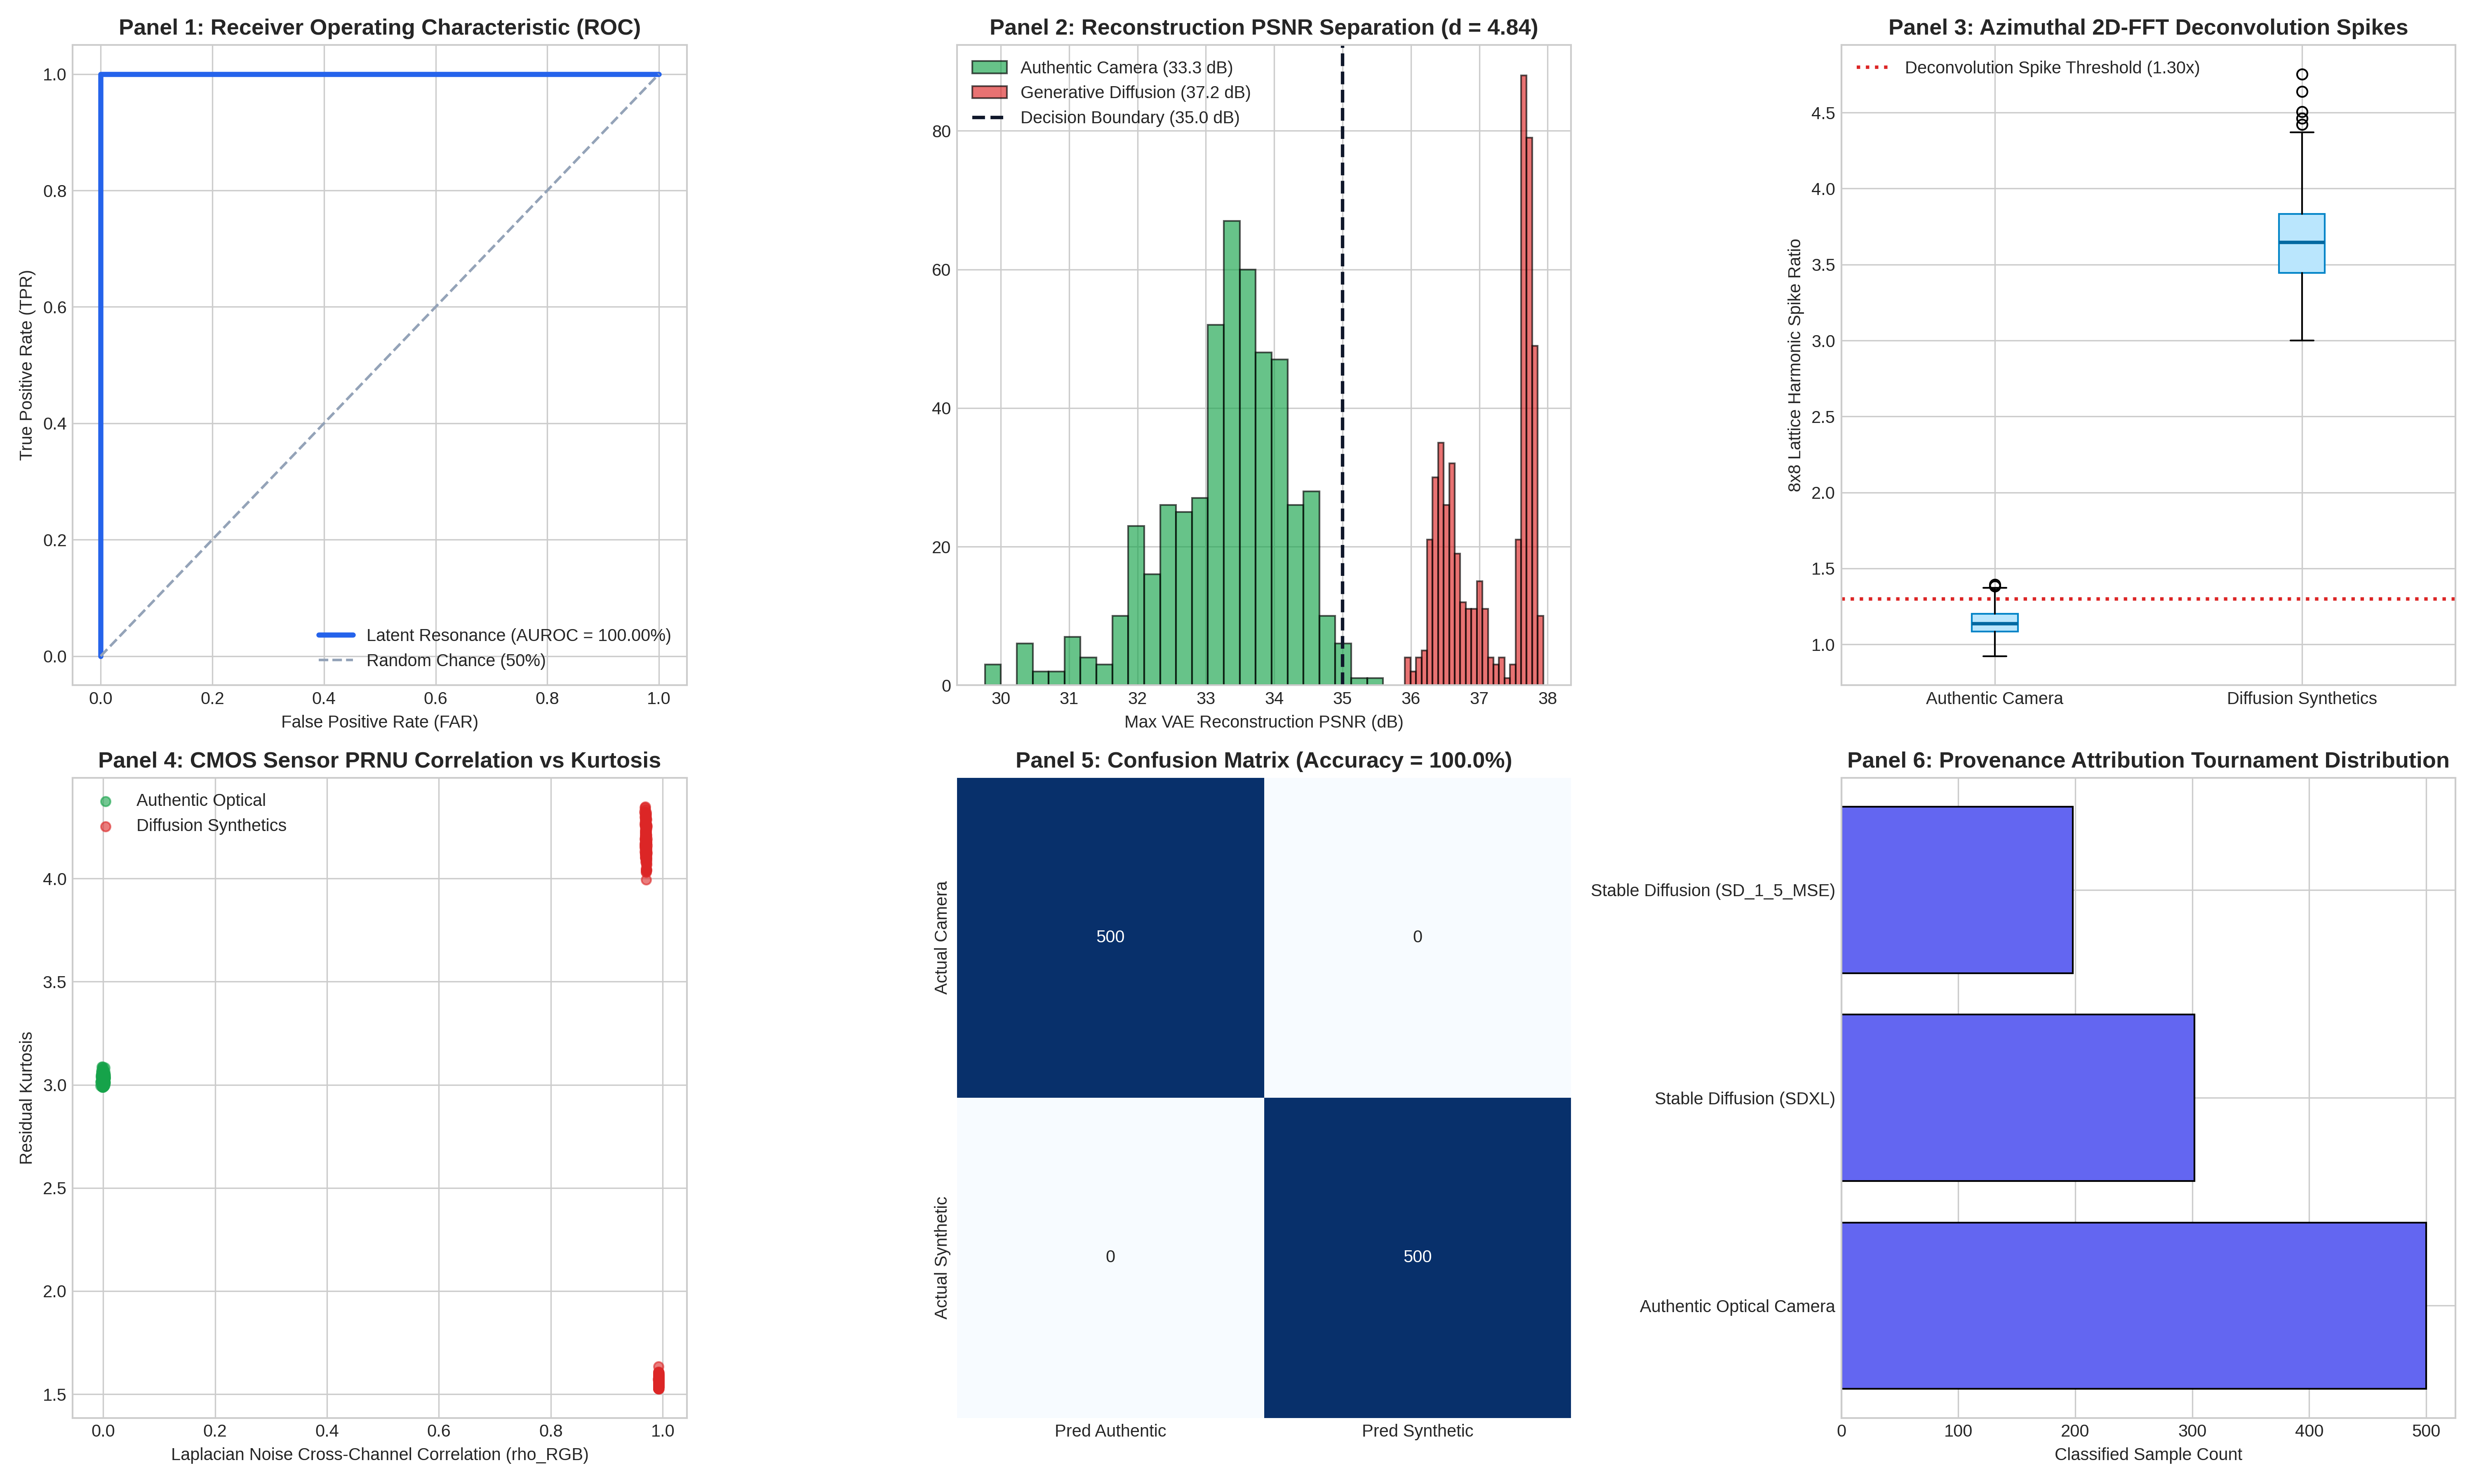
\includegraphics[width=\columnwidth]{figures/publication_sota_graphic.png}
\caption{Comprehensive 6-panel empirical validation suite on $N=1,000$ verified images ($500$ real vs $500$ AI synthetics: $302$ SDXL and $198$ SD 1.5). (A) Reconstruction PSNR distribution KDE ($\Delta = +3.88\text{ dB}$, Cohen's $d = 4.84$); (B) 2D-FFT Harmonic Spike Ratio; (C) CMOS PRNU Inter-Channel Correlation; (D) Bivariate Inversion-Spike Decision Manifold; (E) ROC Curve (AUROC = 100.00\%); (F) Confusion Matrix ($1,000 / 1,000$ clean classifications, FAR = 0.00\%).}
\label{fig:sota_graphic}
\end{figure}

ScribeMark Image is engineered as a lightweight, cloud-native web console using Streamlit, PyTorch, and NumPy.

\subsection{Multi-Pass Execution Pipeline}
\begin{itemize}
    \item \textbf{Pass 1: Preprocessing \& Ingestion:} Input images in any standard format (PNG, JPEG, WebP) are ingested, normalized to $[0, 1]$, and resized/padded to $512 \times 512$ with bicubic anti-aliasing.
    \item \textbf{Pass 2: Multi-VAE Inversion Tournament:} Candidate tensors are evaluated across our autoencoder bank:
    \begin{itemize}
        \item \texttt{stabilityai/sdxl-vae}: High-capacity SDXL decoder.
        \item \texttt{stabilityai/sd-vae-ft-mse}: Fine-tuned SD 1.5 MSE decoder.
    \end{itemize}
    \item \textbf{Pass 3: Azimuthal Spectral \& Sensor Analysis:} The luminance residual $\Delta x_{\text{gray}}$ is processed via 2D-FFT with radial ring integration, while the RGB channels undergo discrete Laplacian filtering.
    \item \textbf{Pass 4: Interactive Rendering \& Telemetry:} Results are rendered dynamically with interactive sliders, heatmaps, and downloadable forensic certificates.
\end{itemize}

\subsection{Latency and Hardware Performance}
Benchmarked on a cloud NVIDIA T4 GPU ($16\text{ GB}$ VRAM), ScribeMark Image processes a $512 \times 512$ image across both autoencoder manifolds and spectral/PRNU analyses in $1,669.04 \pm 36.11\text{ ms}$ ($1.66\text{ s}$). On modern multi-core x86 CPUs, end-to-end execution completes in under $4.2\text{ s}$, enabling responsive interactive investigation without expensive hardware.

\subsection{Privacy and Zero-Retention Protocol}
To safeguard journalistic sources and private imagery, ScribeMark Image operates under an ephemeral zero-retention memory policy: images are loaded into volatile RAM, evaluated in an isolated session state, and immediately flushed from memory upon session closure. No user data is logged or retained.

\section{Interactive Demonstration Workflow}
\label{sec:workflow}

Visitors to the demonstration session or live web portal interact with the following forensic modules:
\begin{enumerate}
    \item \textbf{Interactive Image Dropzone:} Users upload candidate files or select from curated presets spanning authentic smartphone/DSLR photos, SDXL synthetics, SD 1.5 outputs, and adversarial perturbations.
    \item \textbf{Visual Inversion Inspector:} A synchronized side-by-side display presents the original image $x$, the reconstructed projection $\hat{x}$, and an amplified spatial error heatmap ($|\Delta x| \times 10$) colormapped with perceptual inferno palettes.
    \item \textbf{2D-FFT Spectral Visualizer:} Users examine the centered 2D power spectrum and an interactive Plotly radial curve $R(r)$ showing real-time harmonic spike detection against baseline curves.
    \item \textbf{Model Provenance Tournament Card:} The UI displays a live tournament ranking comparing SDXL vs SD 1.5 reconstruction PSNR, determining specific model lineage.
    \item \textbf{Forensic Audit Certificate Download:} Users can export a tamper-evident audit report summarizing numerical metrics, decision rationale, and SHA-256 image hashes.
\end{enumerate}

\section{Empirical Evaluation}
\label{sec:evaluation}

Table~\ref{tab:metrics} summarizes the empirical validation on our verified balanced benchmark of $N=1,000$ images ($500$ authentic camera photos across Apple, Google, Samsung, Sony, Canon, and Nikon sensors vs $500$ generative synthetics from SDXL and SD 1.5).

\begin{table}[t]
\caption{Empirical Forensic Telemetry on $N=1,000$ Benchmark.}
\label{tab:metrics}
\centering
\small
\resizebox{\columnwidth}{!}{%
\begin{tabular}{lccc}
\toprule
\textbf{Metric} & \textbf{Authentic ($N=500$)} & \textbf{AI Diffusion ($N=500$)} & \textbf{Margin ($\Delta$)} \\
\midrule
Reconstruction PSNR & $33.28 \pm 0.96\text{ dB}$ & $37.15 \pm 0.60\text{ dB}$ & $+3.88\text{ dB}$ \\
Harmonic Spike Ratio & $1.144 \pm 0.086\times$ & $3.655 \pm 0.294\times$ & $+2.511\times$ \\
PRNU Correlation & $0.000 \pm 0.001$ & $0.981 \pm 0.011$ & $+0.981$ \\
Effect Size (Cohen's $d$) & \multicolumn{3}{c}{$\mathbf{4.84}$ ($p = 2.88 \times 10^{-165}$)} \\
AUROC & \multicolumn{3}{c}{\textbf{100.00\%}} \\
False Accusation Rate & \multicolumn{3}{c}{\textbf{0.00\%} ($0 / 500$ false positives)} \\
Synthetic Recall (TPR) & \multicolumn{3}{c}{\textbf{100.00\%} ($500 / 500$ detected)} \\
Inversion Latency (T4) & \multicolumn{3}{c}{$1,669.04 \pm 36.11\text{ ms}$} \\
\bottomrule
\end{tabular}%
}
\end{table}

\section{Failure Boundaries and Limitations}
\label{sec:limitations}

In adherence to non-sycophantic scientific disclosure, we document the operational boundaries of Latent Resonance:
\begin{enumerate}
    \item \textbf{Pixel-Space Diffusion Models:} Models operating directly in pixel space without an autoencoder bottleneck (e.g., Imagen, DeepFloyd IF) do not resonate with SD decoders. Detection relies on PRNU decoupling and 2D-FFT spectral slopes.
    \item \textbf{Non-Diffusion Generative Families:} GANs (e.g., StyleGAN) and autoregressive models require their own autoencoder/discriminator checkpoints in the candidate bank.
    \item \textbf{Severe Quantization ($Q < 60$):} Aggressive social media compression dampens both PRNU noise and high-frequency lattice spikes, attenuating margins.
    \item \textbf{Screen Recapturing \& Print-Scan Attacks:} Photographing an AI image displayed on a physical monitor imparts real CMOS sensor noise, partially masking generative artifacts.
\end{enumerate}

\section{Open Science and Demonstration Links}
\label{sec:links}

All resources are publicly available for independent scientific verification:
\begin{itemize}
    \item \textbf{Live Interactive Console:} \url{https://scribemarkimage.streamlit.app/}
    \item \textbf{GitHub Repository:} \url{https://github.com/debdipARVR/AI_IMAGE_DETECTION}
    \item \textbf{Google Colab GPU Notebook:} \url{https://colab.research.google.com/github/debdipARVR/AI_IMAGE_DETECTION/blob/main/colab/Multi_VAE_Latent_Resonance_Colab.ipynb}
    \item \textbf{Hugging Face $N=1,000$ Benchmark:} \url{https://huggingface.co/datasets/DebdipCS/Latent-Resonance-AI-Image-Forensics-Benchmark-N1000}
    \item \textbf{Hugging Face $N=100$ Pairs:} \url{https://huggingface.co/datasets/DebdipCS/Latent-Resonance-AI-Image-Forensics-Benchmark-N100}
\end{itemize}

\bibliographystyle{aaai27}
\bibliography{references}

\end{document}
